\subsection{Esperimento 3: variazione della dinamicità dell'ambiente}\label{subsec:exp3}
Fino ad ora gli esperimenti effettuati hanno usato valori di $\mathbb{P_D}$ e $\mathbb{P_B}$ coerenti con un contesto in cui l'informazione relativa al livello di esplorazione in una regione rimane attendibile per un intervallo di tempo relativamente lungo, ovvero coerenti con ambienti aventi bassa dinamicità. 
Con quest'ultimo esperimento dunque si vuole verificare le performance del sistema quando opera in un ambiente maggiormente mutabile nel tempo.
Dati i risultati del precedente esperimento, si è deciso di eseguire queste simulazioni usando solamente la ricerca \textit{local}, confrontando nelle varie prove lo stesso scenario iniziale, ma variando le probabilità di apparizione e disconnessione degli utenti: in un caso si usano i valori definiti in \ref{sec:param_vals}, mentre nell'altro si usano $\mathbb{P_D}=0.01$ e $\mathbb{P_B}=0.07$.

\begin{figure}[p]
    \centering
    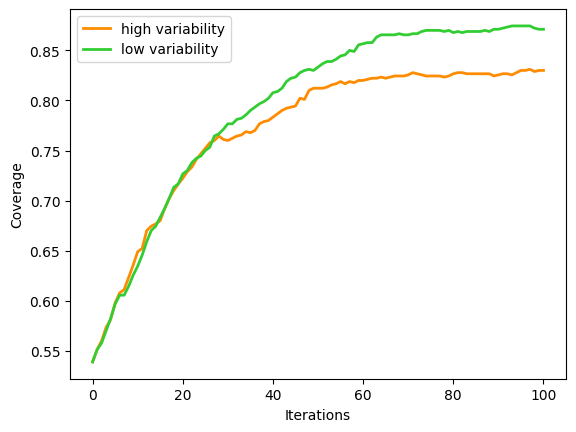
\includegraphics[width=0.8\textwidth]{img/ch4/experiment3/coverages_graphic_comparison.png}
    \caption[Grafici di copertura nel terzo esperimento]{Confronto tra l'andamento medio della copertura negli scenari di simulazione del terzo esperimento.}
    \label{fig:confronto_cov_exp3}

\vspace*{0.5cm}

    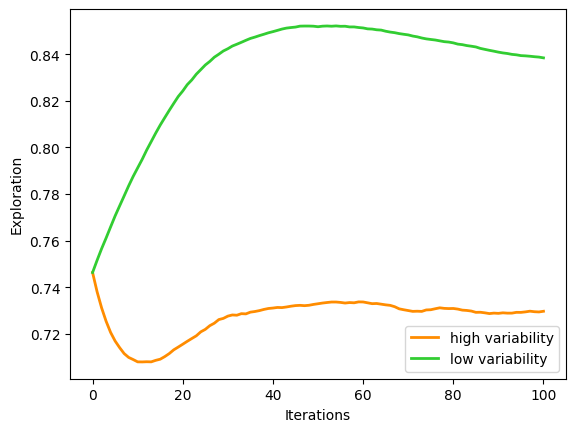
\includegraphics[width=0.8\textwidth]{img/ch4/experiment3/exploration_graphic_comparison.png}
    \caption[Grafici di esplorazione nel terzo esperimento]{Confronto tra l'andamento medio dell'esplorazione negli scenari di simulazione del terzo esperimento.}
    \label{fig:confronto_expl_exp3}
\end{figure}

Analizzando i risultati in Figura \ref{fig:confronto_expl_exp3} notiamo come i livelli di \textbf{esplorazione} diminuiscano drasticamente: questo tuttavia era prevedibile, infatti con questa configurazione la probabilità che appaia un utente in una cella cresce molto rapidamente, e rende impossibile raggiungere alti livelli di esplorazione con la quantità di agenti usati nelle simulazioni.
Per quanto riguarda la \textbf{copertura} (Figura \ref{fig:confronto_cov_exp3}) invece, si riescono a raggiungere dei livelli abbastanza buoni: benché l'algoritmo di esplorazione non impedisca di esplorare ripetutamente alcune zone, è abbastanza flessibile da guidare gli agenti attraverso l'area, disincentivando spostamenti brevi e ripetuti in favore di una traiettoria più pulita.

\begin{figure}
    \centering
    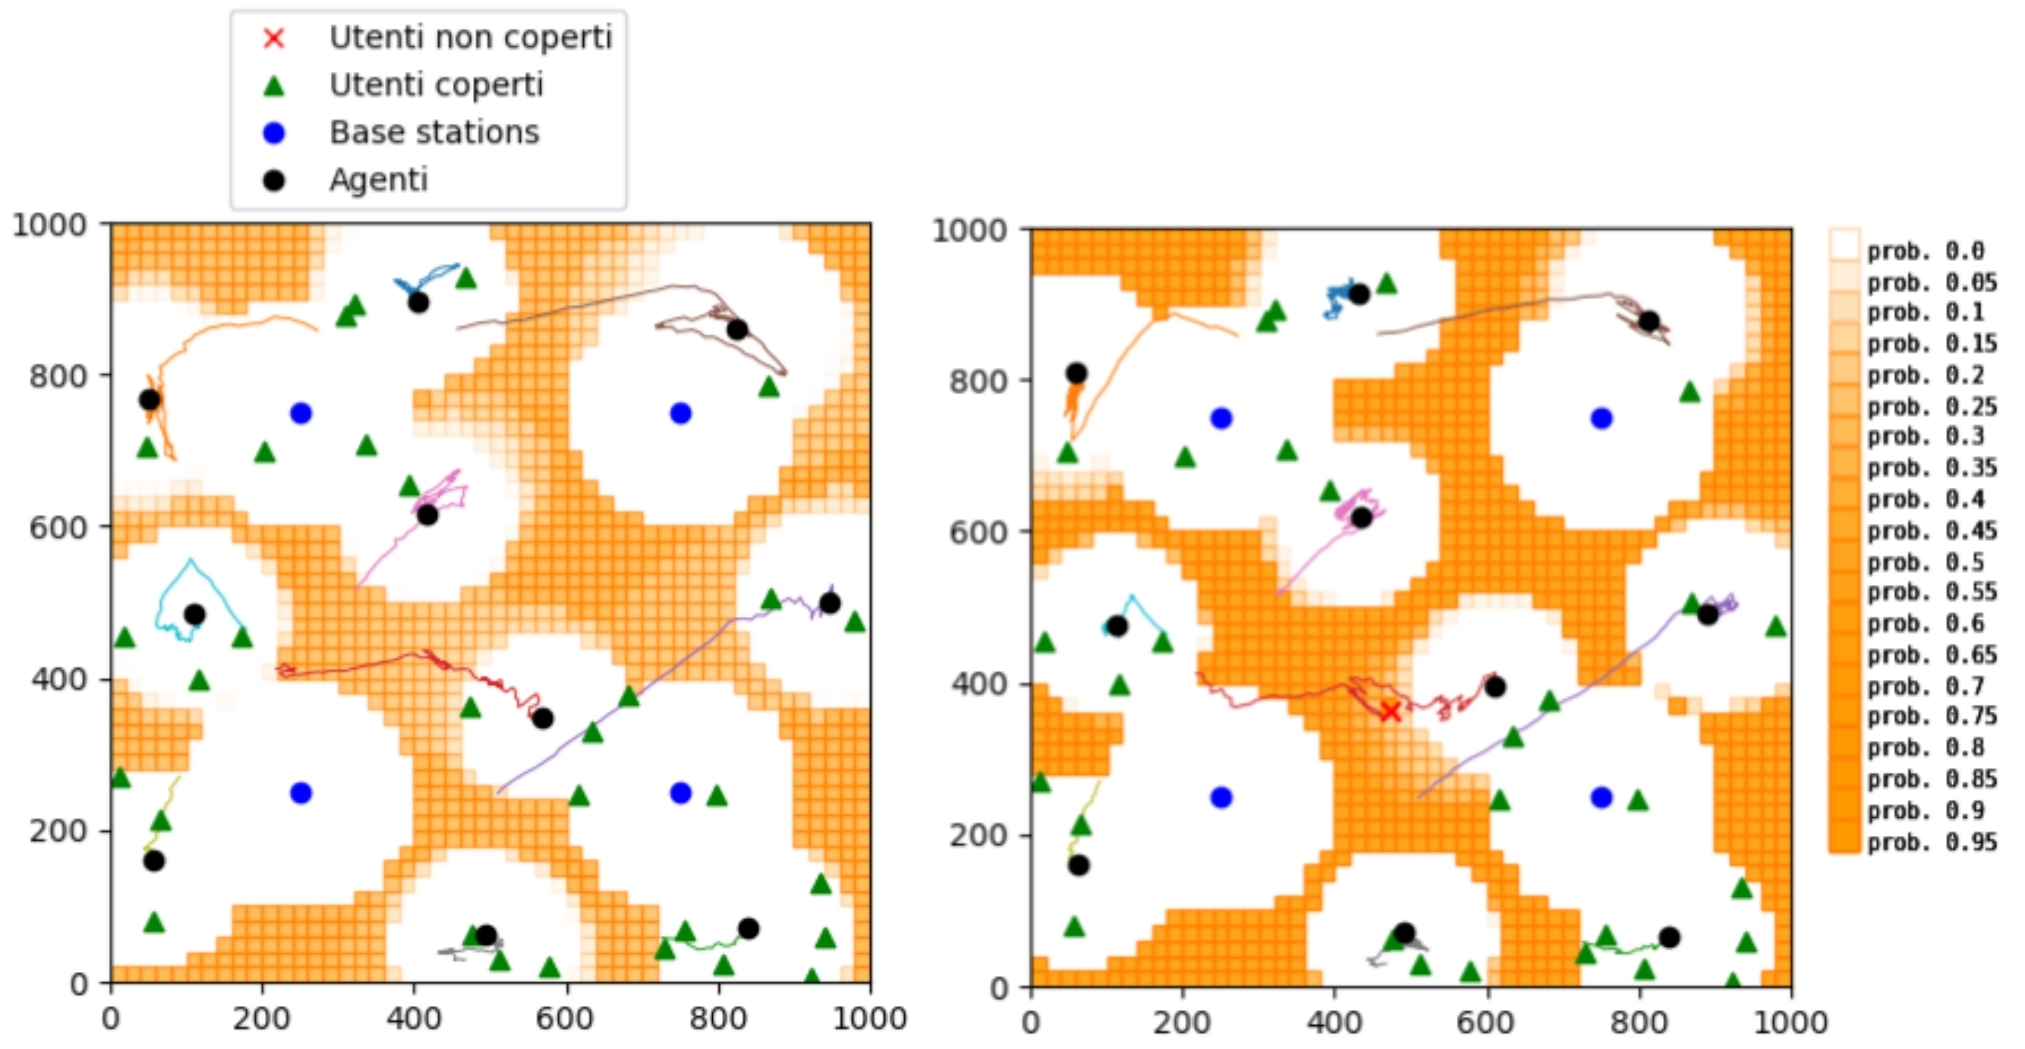
\includegraphics[width=1\linewidth]{img/ch4/experiment3/esempio_exp3_1.jpg}
    \label{fig:esempio_exp3_1}

    \vspace*{0.5cm}
    
    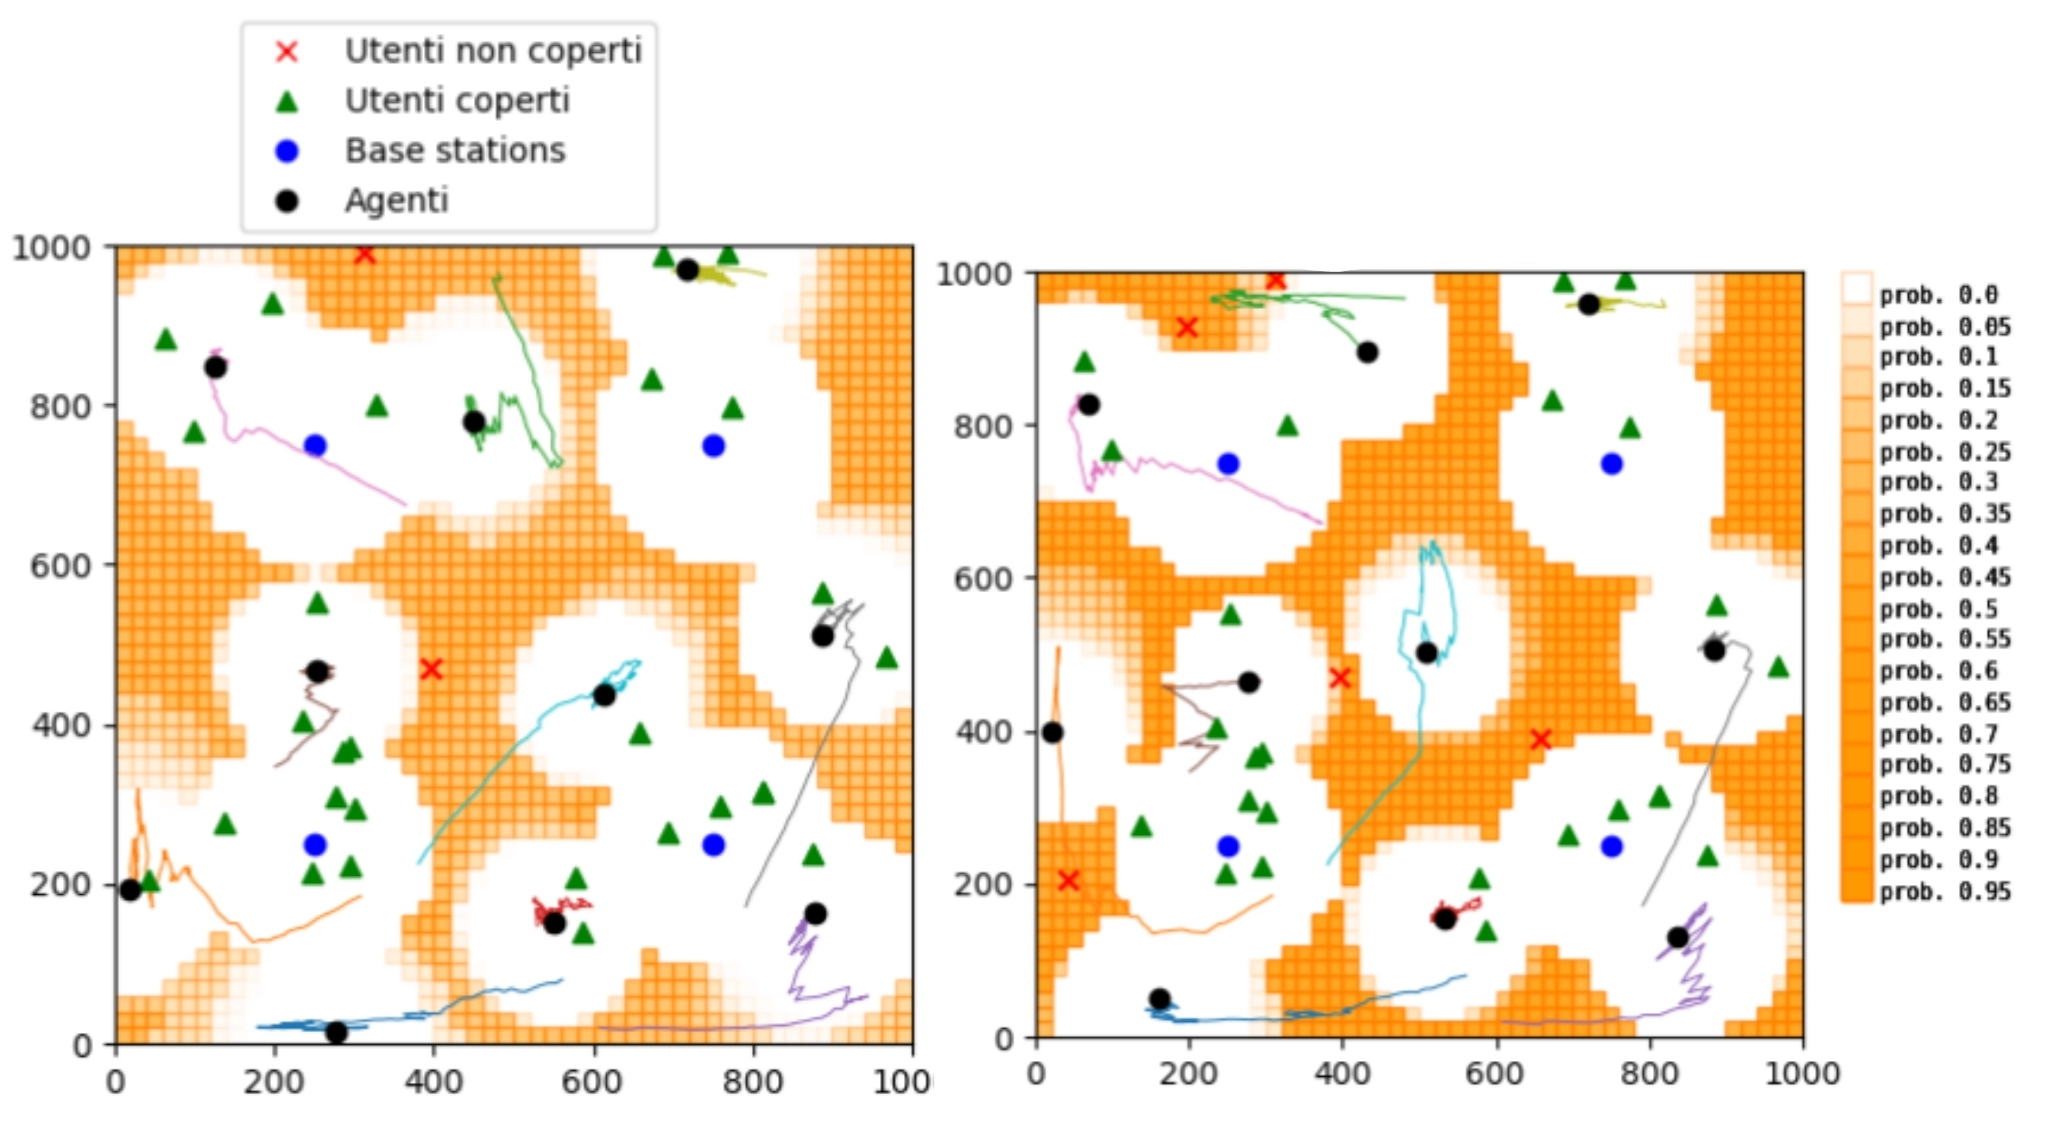
\includegraphics[width=1\linewidth]{img/ch4/experiment3/esempio_exp3_2.jpg}
    \label{fig:esempio_exp3_2}
    \caption[Confronti tra simulazioni con probabilità diverse]{Confronti tra simulazioni con probabilità diverse. Nello scenario di simulazione in alto, nonostante il cambio di parametri le due prove hanno raggiunto livelli di copertura simili. Nello scenario in basso invece la maggiore variabilità dell'ambiente provoca una diminuzione dei risultati raggiunti.}
    
    
\end{figure}